% -*- mode: noweb; noweb-default-code-mode: R-mode; -*-

\documentclass[a4paper]{article}


\usepackage[pdftex,
bookmarks,
bookmarksopen,
pdfauthor={Per Broberg},
pdftitle={Samroc example}]{hyperref}



% \VignetteIndexEntry{A package for retrieval, preparation and analysis of data from the Affymetrix GeneChip.}
% \VignetteDepends{SAGx, multtest}
% \VignetteKeyword{samroc}
% \VignettePackage{SAGx}

\usepackage[authoryear,round]{natbib}

\usepackage{C:/R/rw2001/share/texmf/Sweave}
\begin{document}

\title{Using functions \textit{samrocNboot} and \textit{pava.fdr}}

\author{Per Broberg} 

\maketitle

\section*{Analysis of the data from Golub \ital{et al.}}

Consider the microarray experiment in \cite{golubetal} where ALL and AML types are compared.
The data are available within package \textit{multtest}. We can analyse those data in SAGx  with the function \textit{samrocNboot}. The ideas behind
it are presented in \cite{broberg:2003}. Briefly, the method relies on a penalised \textit{t}-test statistica $ d = (\bar{x}_1 - \bar{x}_2)/(S + a)$ \cite{efron:2001}. Example code now follows 

\begin{Schunk}
\begin{Sinput}
> library(multtest)
> data(golub)
> samroc.res <- samrocNboot(data = golub, formula = ~as.factor(golub.cl))
> samroc.res$p0
\end{Sinput}
\begin{Soutput}
[1] 0.3756356
\end{Soutput}
\end{Schunk}
The function \textit{samrocNboot} is used to perform a penalised \textit{t}-test. The estimated
proportion unchanged genes equals 0.38. The distribution of \textit{p}-values is shown in Figure~\ref{hist1},
which vindicates that many genes are changed. Furthermore, using the function \textit{pava.fdr} we obtain estimates of the FDR and 
of the local FDR, see Figure~\ref{hist2}. This function is presented in \cite{broberg:2004} and combines the local FDR estimator 
of \cite{aubert:2004} with Poisson regression (see \cite{efron:2004}) and isotonic regression.


\begin{figure}[htbp]
\centering

\begin{Schunk}
\begin{Sinput}
> par(bg = "cornsilk")
> hist(samroc.res$pvalue, xlab = "p-value", main = "", col = "orange", 
+     freq = F)
> print(abline(samroc.res$p0, 0, col = "red"))
\end{Sinput}
\begin{Soutput}
NULL
\end{Soutput}
\end{Schunk}
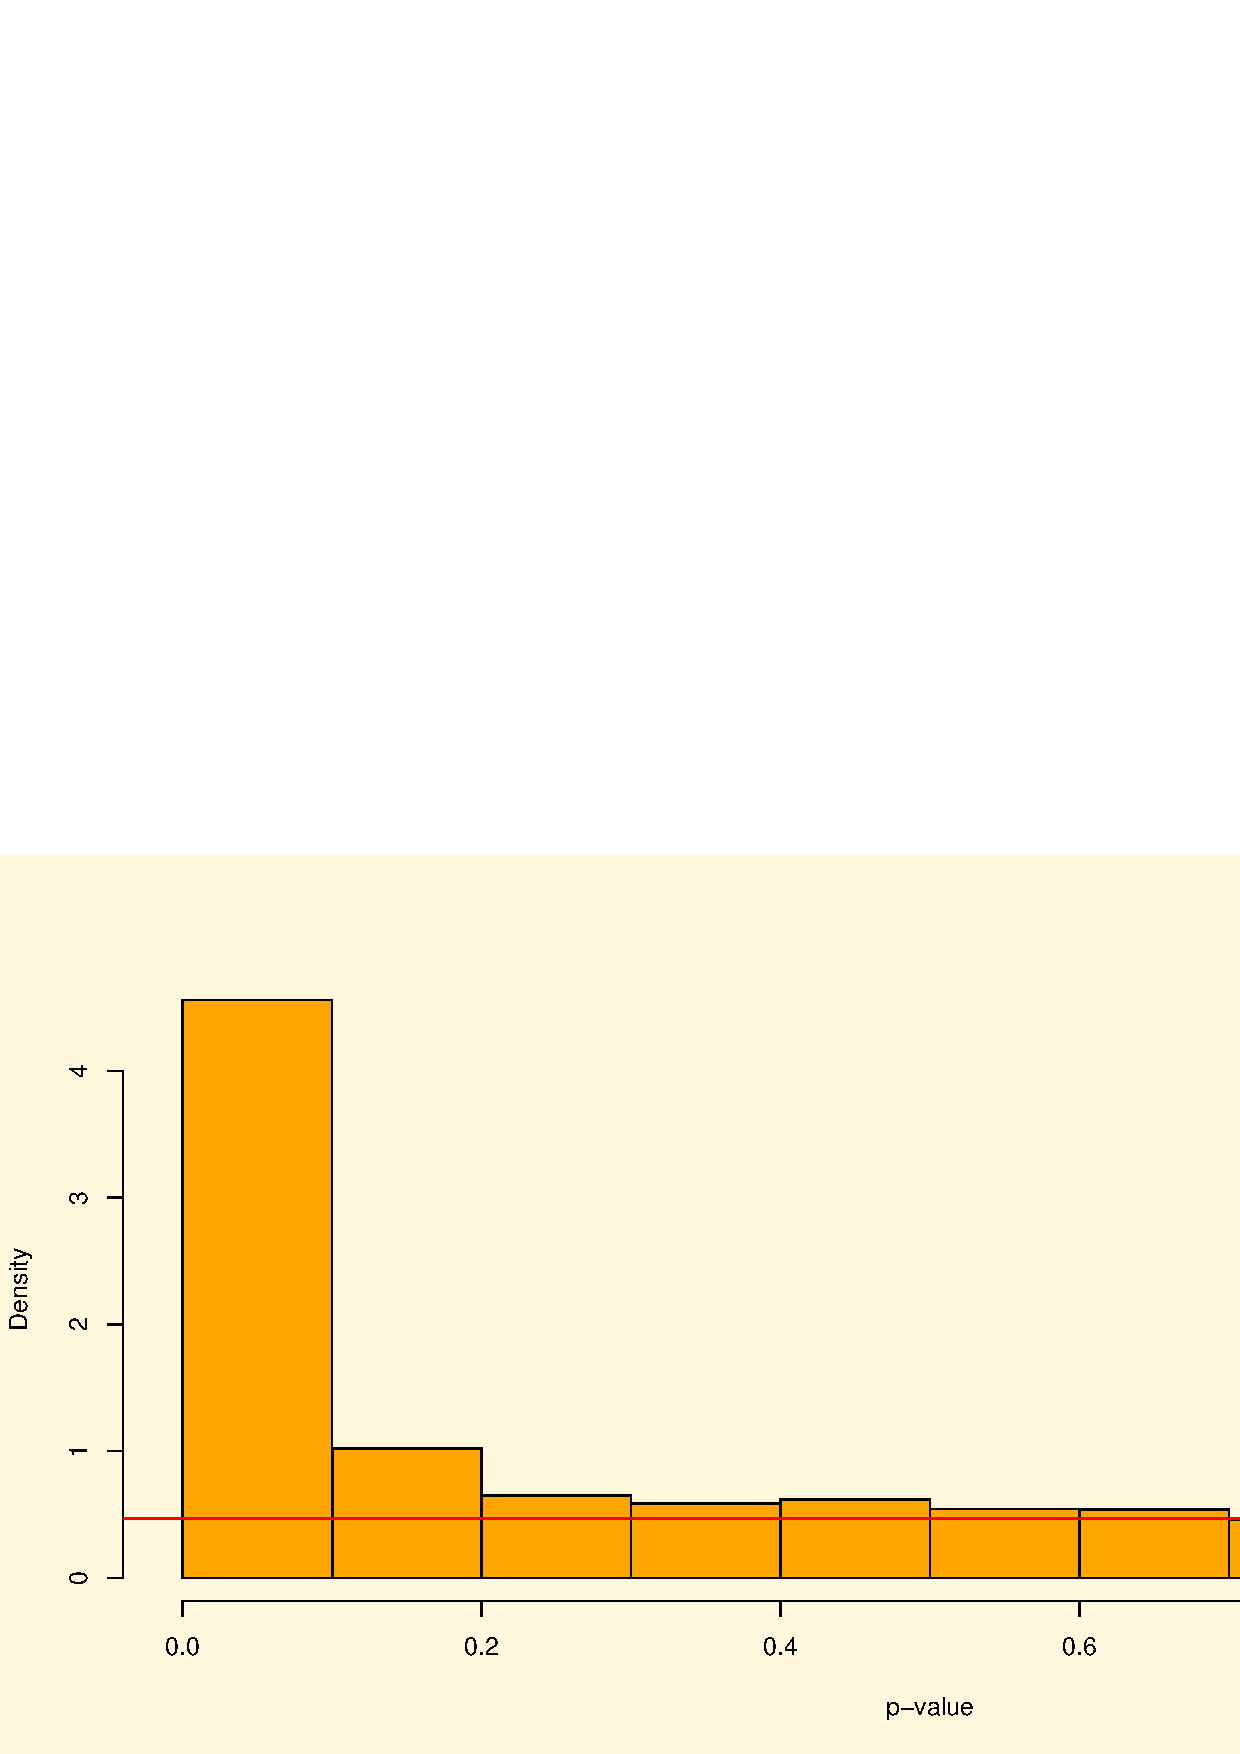
\includegraphics{samroc-ex-002}
\caption{Histogram of the \textit{p}-values generated by function \textit{samrocNboot}}
\label{hist1}
\end{figure}

\begin{figure}[htbp]
\centering
\begin{Schunk}
\begin{Sinput}
> par(bg = "cornsilk")
> fdrs <- pava.fdr(ps = samroc.res$pvalues)
> plot(samroc.res$pvalues, fdrs$pava.local.fdr, type = "n", xlab = "p-value", 
+     ylab = "False Discovery Rate (FDR)")
> lines(lowess(samroc.res$pvalues, fdrs$pava.local.fdr), col = "red")
> lines(lowess(samroc.res$pvalues, fdrs$pava.fdr), col = "blue")
> legend(0.1, 0.9, pch = NULL, col = c("red", "blue"), c("pava local FDR", 
+     "pava FDR"), lty = 1)
\end{Sinput}
\end{Schunk}
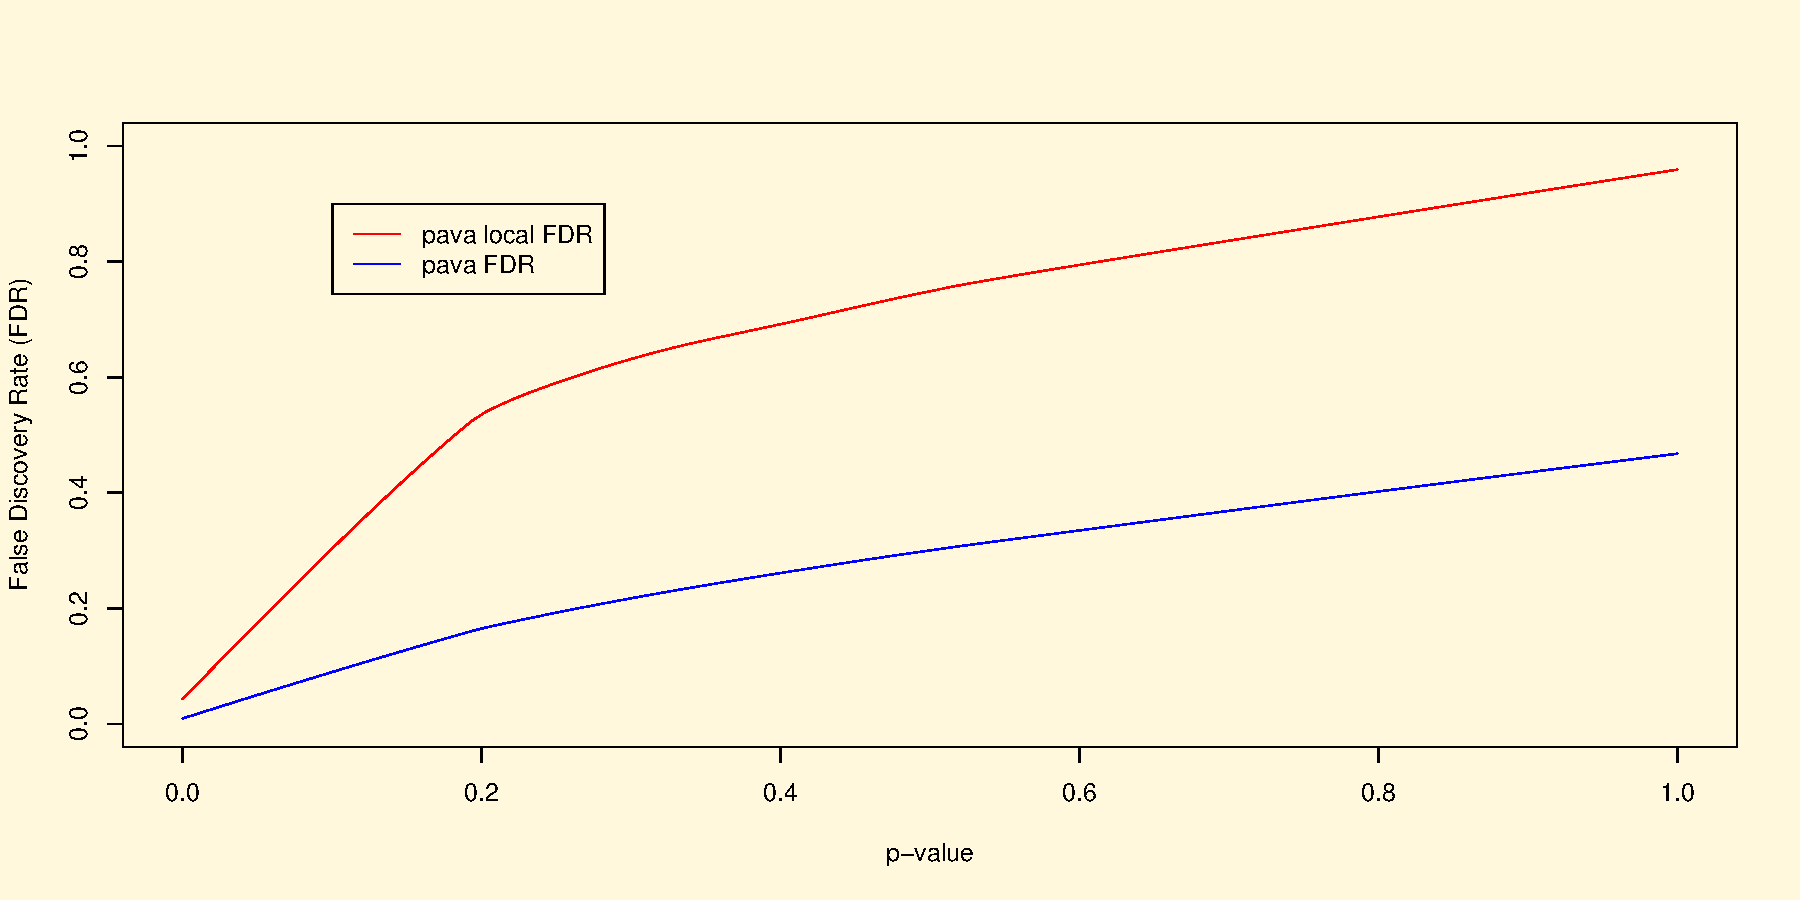
\includegraphics{samroc-ex-003}
\caption{Scatter plot of the local false discovery rate and the false discovery rate as estimated by function \textit{pava.fdr}}
\label{hist2}
\end{figure}

%%%%%%%%%%%%%%%%%%%%%%%%%%%%%%%%%%%%%%
\newpage
\bibliographystyle{plainnat}
\bibliography{samroc-ex}
%%%%%%%%%%%%%%%%%%%%%%%%%%%%%%%%%%

\end{document}
